% Options for packages loaded elsewhere
\PassOptionsToPackage{unicode}{hyperref}
\PassOptionsToPackage{hyphens}{url}
\PassOptionsToPackage{dvipsnames,svgnames,x11names}{xcolor}
%
\documentclass[
  10pt,
  dvipsnames,enabledeprecatedfontcommands]{scrartcl}
\title{Appendix: confirmation measures and the difficulty about
conjunction}
\author{Marcello Di Bello and Rafal Urbaniak}
\date{}

\usepackage{amsmath,amssymb}
\usepackage{lmodern}
\usepackage{iftex}
\ifPDFTeX
  \usepackage[T1]{fontenc}
  \usepackage[utf8]{inputenc}
  \usepackage{textcomp} % provide euro and other symbols
\else % if luatex or xetex
  \usepackage{unicode-math}
  \defaultfontfeatures{Scale=MatchLowercase}
  \defaultfontfeatures[\rmfamily]{Ligatures=TeX,Scale=1}
\fi
% Use upquote if available, for straight quotes in verbatim environments
\IfFileExists{upquote.sty}{\usepackage{upquote}}{}
\IfFileExists{microtype.sty}{% use microtype if available
  \usepackage[]{microtype}
  \UseMicrotypeSet[protrusion]{basicmath} % disable protrusion for tt fonts
}{}
\usepackage{xcolor}
\IfFileExists{xurl.sty}{\usepackage{xurl}}{} % add URL line breaks if available
\IfFileExists{bookmark.sty}{\usepackage{bookmark}}{\usepackage{hyperref}}
\hypersetup{
  pdftitle={Appendix: confirmation measures and the difficulty about conjunction},
  pdfauthor={Marcello Di Bello and Rafal Urbaniak},
  colorlinks=true,
  linkcolor={Maroon},
  filecolor={Maroon},
  citecolor={Blue},
  urlcolor={blue},
  pdfcreator={LaTeX via pandoc}}
\urlstyle{same} % disable monospaced font for URLs
\usepackage{graphicx}
\makeatletter
\def\maxwidth{\ifdim\Gin@nat@width>\linewidth\linewidth\else\Gin@nat@width\fi}
\def\maxheight{\ifdim\Gin@nat@height>\textheight\textheight\else\Gin@nat@height\fi}
\makeatother
% Scale images if necessary, so that they will not overflow the page
% margins by default, and it is still possible to overwrite the defaults
% using explicit options in \includegraphics[width, height, ...]{}
\setkeys{Gin}{width=\maxwidth,height=\maxheight,keepaspectratio}
% Set default figure placement to htbp
\makeatletter
\def\fps@figure{htbp}
\makeatother
\setlength{\emergencystretch}{3em} % prevent overfull lines
\providecommand{\tightlist}{%
  \setlength{\itemsep}{0pt}\setlength{\parskip}{0pt}}
\setcounter{secnumdepth}{5}
%\documentclass{article}

% %packages
\usepackage{booktabs}
\usepackage[left]{showlabels}
\usepackage{multirow}
\usepackage{subcaption}

\usepackage{graphicx}
\usepackage{longtable}
\usepackage{ragged2e}
\usepackage{etex}
%\usepackage{yfonts}
\usepackage{marvosym}
\usepackage[notextcomp]{kpfonts}
\usepackage{nicefrac}
\newcommand*{\QED}{\hfill \footnotesize {\sc Q.e.d.}}
\usepackage{floatrow}

\usepackage[textsize=footnotesize]{todonotes}
\newcommand{\ali}[1]{\todo[color=gray!40]{\textbf{Alicja:} #1}}
\newcommand{\mar}[1]{\todo[color=blue!40]{#1}}
\newcommand{\raf}[1]{\todo[color=olive!40]{#1}}

%\linespread{1.5}
\newcommand{\indep}{\!\perp \!\!\! \perp\!}


\setlength{\parindent}{10pt}
\setlength{\parskip}{1pt}


%language
%\usepackage{times}
\usepackage{mathptmx}
\usepackage[scaled=0.86]{helvet}
\usepackage{t1enc}
%\usepackage[utf8x]{inputenc}
%\usepackage[polish]{babel}
%\usepackage{polski}




%AMS
\usepackage{amsfonts}
\usepackage{amssymb}
\usepackage{amsthm}
\usepackage{amsmath}
\usepackage{mathtools}

\usepackage{geometry}
 \geometry{a4paper,left=35mm,top=20mm,}


%environments
\newtheorem{fact}{Fact}



%abbreviations
\newcommand{\ra}{\rangle}
\newcommand{\la}{\langle}
\newcommand{\n}{\neg}
\newcommand{\et}{\wedge}
\newcommand{\jt}{\rightarrow}
\newcommand{\ko}[1]{\forall  #1\,}
\newcommand{\ro}{\leftrightarrow}
\newcommand{\exi}[1]{\exists\, {_{#1}}}
\newcommand{\pr}[1]{\ensuremath{\mathsf{P}(#1)}}
\newcommand{\cost}{\mathsf{cost}}
\newcommand{\benefit}{\mathsf{benefit}}
\newcommand{\ut}{\mathsf{ut}}

\newcommand{\odds}{\mathsf{Odds}}
\newcommand{\ind}{\mathsf{Ind}}
\newcommand{\nf}[2]{\nicefrac{#1\,}{#2}}
\newcommand{\R}[1]{\texttt{#1}}
\newcommand{\prr}[1]{\mbox{$\mathtt{P}_{prior}(#1)$}}
\newcommand{\prp}[1]{\mbox{$\mathtt{P}_{posterior}(#1)$}}



\newtheorem{q}{\color{blue}Question}
\newtheorem{lemma}{Lemma}
\newtheorem{theorem}{Theorem}
\newtheorem{corollary}{Corollary}[fact]


%technical intermezzo
%---------------------

\newcommand{\intermezzoa}{
	\begin{minipage}[c]{13cm}
	\begin{center}\rule{10cm}{0.4pt}



	\tiny{\sc Optional Content Starts}
	
	\vspace{-1mm}
	
	\rule{10cm}{0.4pt}\end{center}
	\end{minipage}\nopagebreak 
	}


\newcommand{\intermezzob}{\nopagebreak 
	\begin{minipage}[c]{13cm}
	\begin{center}\rule{10cm}{0.4pt}

	\tiny{\sc Optional Content Ends}
	
	\vspace{-1mm}
	
	\rule{10cm}{0.4pt}\end{center}
	\end{minipage}
	}
	
	
%--------------------






















\newtheorem*{reply*}{Reply}
\usepackage{enumitem}
\newcommand{\question}[1]{\begin{enumerate}[resume,leftmargin=0cm,labelsep=0cm,align=left]
\item #1
\end{enumerate}}

\usepackage{float}

% \setbeamertemplate{blocks}[rounded][shadow=true]
% \setbeamertemplate{itemize items}[ball]
% \AtBeginPart{}
% \AtBeginSection{}
% \AtBeginSubsection{}
% \AtBeginSubsubsection{}
% \setlength{\emergencystretch}{0em}
% \setlength{\parskip}{0pt}






\usepackage[authoryear]{natbib}

%\bibliographystyle{apalike}



\usepackage{tikz}
\usetikzlibrary{positioning,shapes,arrows}

\usepackage{booktabs}
\usepackage{longtable}
\usepackage{array}
\usepackage{multirow}
\usepackage{wrapfig}
\usepackage{float}
\usepackage{colortbl}
\usepackage{pdflscape}
\usepackage{tabu}
\usepackage{threeparttable}
\usepackage{threeparttablex}
\usepackage[normalem]{ulem}
\usepackage{makecell}
\usepackage{xcolor}
\ifLuaTeX
  \usepackage{selnolig}  % disable illegal ligatures
\fi

\begin{document}
\maketitle

\tableofcontents

\hypertarget{bayesian-networks-and-probabilistic-independence}{%
\subsection*{Bayesian networks and probabilistic
independence}\label{bayesian-networks-and-probabilistic-independence}}
\addcontentsline{toc}{subsection}{Bayesian networks and probabilistic
independence}

One assumption often made in the formulation of the conjunction paradox
is that claims \(A\) and \(B\) are probabilistically independent. This
is not always the case---we have seen that the paradox does subside even
if the two claims are dependent. However, two fairly natural set-ups for
conjunctive hypotheses and evidence supporting them (Figure
\ref{fig:conjunctionBNs}) indeed do have some independencies built in,
and so it is also natural what can be said about the conjunction problem
given these independencies. Moreover, in some context, we will be freely
using the independence assumptions, as a counterexample to a general
claim still remains one even if it satisfies an additional requirement,
that is, independence conditions.

We will be considering the conjunction of two hypotheses, \(A\) and
\(B\), their respective pieces of evidence \(a\) and \(b\), and their
conjunction \(AB\), in two set-ups, illustrated by the Bayesian networks
shown in Figure \ref{fig:conjunctionBNs}. The key difference here is
that we allow direct dependence between the hypotheses in the second
network. In both Bayesian networks, the CPT for the conjunction
trivially mirrors the one for conjunction, as in Table
\ref{tab:CPTconjunction2}.

\vspace{1mm}
\footnotesize

\normalsize

\begin{figure}[H]
\hspace{2mm}\scalebox{1}{\begin{subfigure}[!ht]{0.45\textwidth}

\begin{center}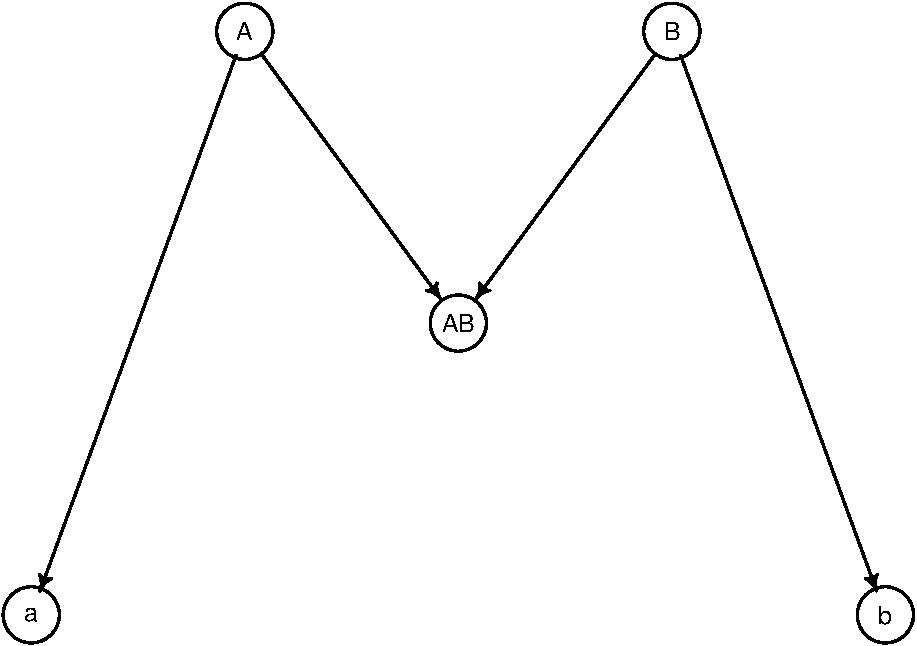
\includegraphics[width=1\linewidth]{conjunction-appendix7_files/figure-latex/unnamed-chunk-2-1} \end{center}
\subcaption{\textsf{DAG1}}
\end{subfigure}} 
\hspace{5mm}\begin{subfigure}[!ht]{0.45\textwidth}
\vspace{1mm}

\begin{center}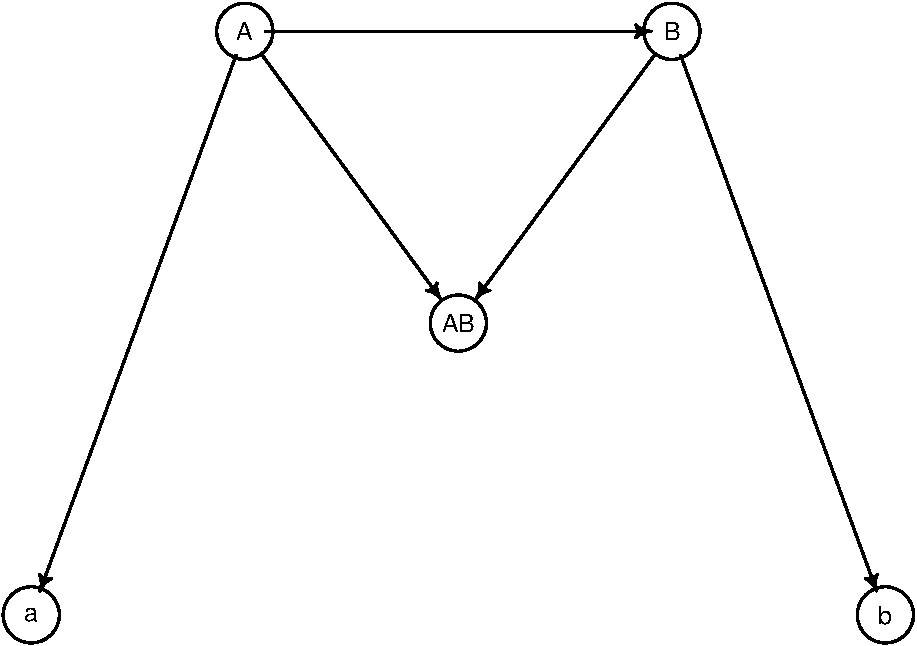
\includegraphics[width=1\linewidth]{conjunction-appendix7_files/figure-latex/unnamed-chunk-3-1} \end{center}
\subcaption{\textsf{DAG2}}
\end{subfigure}
\normalsize
\caption{Two DAGs for the conjunction problem.}
\label{fig:conjunctionBNs}
\end{figure}

\begin{table}[h]
\begin{table}[H]
\centering
\begin{tabular}{lllr}
\toprule
\multicolumn{1}{c}{} & \multicolumn{1}{c}{A} & \multicolumn{1}{c}{B} & \multicolumn{1}{c}{} \\
AB &  &  & Pr\\
\midrule
\cellcolor{gray!6}{1} & \cellcolor{gray!6}{1} & \cellcolor{gray!6}{1} & \cellcolor{gray!6}{1}\\
0 & 1 & 1 & 0\\
\cellcolor{gray!6}{1} & \cellcolor{gray!6}{0} & \cellcolor{gray!6}{1} & \cellcolor{gray!6}{0}\\
0 & 0 & 1 & 1\\
\cellcolor{gray!6}{1} & \cellcolor{gray!6}{1} & \cellcolor{gray!6}{0} & \cellcolor{gray!6}{0}\\
0 & 1 & 0 & 1\\
\cellcolor{gray!6}{1} & \cellcolor{gray!6}{0} & \cellcolor{gray!6}{0} & \cellcolor{gray!6}{0}\\
0 & 0 & 0 & 1\\
\bottomrule
\end{tabular}
\end{table}
\normalsize
\caption{Conditional probability table for the conjunction node.}
\label{tab:CPTconjunction2}
\end{table}

\newpage 
\vspace{1mm}
\footnotesize

\normalsize

Directed Acyclic Graphs (DAGs) are useful for representing graphically
these relationships of independence. The edges, intuitively, are meant
to capture direct influence between the nodes. The role that such direct
influence plays is that in a Bayesian network built over a DAG any node
is conditionally independent of its nondescentants (including
ancestors), given its parents. If this is the case for a given
probabilistic measure \(\pr{}\) and a given DAG, we say that \(\pr{}\)
is compatible with \(\mathsf{G}\), and they can be put together to
constitute a Bayesian network.

The graphical counterpart of probabilistic independence is the so-called
\textbf{d-separation}, \(\indep_d\). We say that two nodes, \(X\) and
\(Y\), are d-separated given a set of nodes
\(\mathsf{Z}\)---\(X\indep_d Y \vert \mathsf{Z}\) --- iff for every
undirected path from \(X\) to \(Y\) there is a node \(Z'\) on the path
such that either:

\begin{itemize} 
\item $Z' \in \mathsf{Z}$ and there is a \emph{serial} connection, $\rightarrow Z' \rightarrow$, on the path,
\item  $Z'\in \mathsf{Z}$ and there is a diverging connection, $\leftarrow Z' \rightarrow $, on the path,
\item There is a connection $\rightarrow Z' \leftarrow$ on the path, and neither $Z'$ nor its descendants are in $\mathsf{Z}$.
\end{itemize}

\vspace{1mm}

Finally, two sets of nodes, \(\mathsf{X}\) and \(\mathsf{Y}\), are
d-separated given \(\mathsf{Z}\) if every node in \(\mathsf{X}\) is
d-separated from every node in \(\mathsf{Y}\) given \(\mathsf{Z}\). With
serial connection, for instance, if:

\footnotesize 
\begin{center}
\begin{tabular}{@{}lp{4.3cm}@{}}\toprule
Node & Proposition \\ \midrule 
$G$ & The suspect is guilty. \\
$B$ & The blood stain comes from the suspect.\\
$M$ & The crime scene stain and the suspect's blood share their DNA profile.\\
\bottomrule
\end{tabular}
\end{center}
\normalsize

\noindent We naturally would like to have the connection
\(G \rightarrow B \rightarrow M\). If we don't know whether \(B\) holds,
\(G\) seems to have an indirect impact on the probability of \(M\). Yet,
once we find out that \(B\) is true, we expect the profile match, and
whether \(G\) holds has no further impact on the probability of \(M\).

Take an example of a diverging connections. Say you have two coins, one
fair, one biased. Conditional on which coin you have chosen, the results
of subsequent tosses are independent. But if you don't know which coin
you have chosen, the result of previous tosses give you some information
about which coin it is, and this has impact on your estimate of the
probability of heads in the next toss. Whether a coin is fair, \(F\) or
not has an impact on the result of the first toss, \(H1\), and on the
result of the second toss, \(H2\). So \(H1 \leftarrow F \rightarrow H2\)
seems to be appropriate. Now, on one hand, as long as we don't know
whether \(F\), \(H1\) increases the probability of \(H2\). On the other,
once we know that \(F\), though, \(H1\) and \(H2\) become independent,
and so conditioning on the parent in a fork makes its childern
independent (provided there is no other open path between them in the
graph).

For converging connections, let \(G\) and \(B\) be as above, and let:

\begin{center}
\begin{tabular}{@{}lp{4.3cm}@{}}\toprule
Node & Proposition \\ \midrule 
$O$ & The crime scene stain comes from the offender.\\
\bottomrule
\end{tabular}
\end{center}
\normalsize

\noindent Both \(G\) and \(O\) influence \(B\). If he's guilty, it's
more likely that the blood stain comes from him, and if the blood crime
stain comes from the offender it is more likely to come from the suspect
(for instance, more so than if it comes from the victim). Moreover,
\(G\) and \(O\) seem independent -- whether the suspect is guilty
doesn't have any bearing on whether the stain comes from the offender.
Thus, a converging connection \(G\rightarrow B \leftarrow O\) seem
appropriate. However, if you do find out that \(B\) is true, that the
stain comes from the suspect, whether the crime stain comes from the
offender becomes relevant for whether the suspect is guilty.

One important reason why d-separation matters is that it can be proven
that if two sets of nodes are d-separated given a third one, then they
are independent given the third one, for any probabilistic measures
compatible with a given DAG. Interestingly, lack of d-separation doesn't
entail dependence for any probabilistic measure compatible with a given
DAG. Rather, it only allows for it: if nodes are d-separated, there is
at least one probabilistic measure fitting the DAG according to which
they are independent. So, at least, no false independence can be
inferred from the DAG, and all the dependencies are built into it.

Now, getting back to the conjunction problem, the d-separations entailed
by these networks differ (examples can be found in Table
\ref{tab:indepBNS})---in fact, \textsf{DAG1} entails 31 d-separations,
while \textsf{DAG2} entails 22 of them. Attention should be paid to the
notation. In the above, variables represent nodes, and so each
d-separation entails a probabilistic statement about all combination of
the node states involved. For instance, assuming each node is binary
with two possible states, 1 and 0, \mbox{$B   \indep_d\,\,  a $} entails
that for any \mbox{$ B_i, a_i \in \{0, 1\}$} we have
\(\pr{B = B_i} = \pr{B = B_i \vert a = a_i}\).

\begin{table}[h]
\begin{tabular}{cr}
\toprule
Bayesian network 1  & Bayesian network 2\\
\midrule
\cellcolor{gray!6}{$A   \indep_d\,\, B  $}&\cellcolor{gray!6}{     $ A  \indep_d\,\, b \vert  B  $} \\
$A   \indep_d\,\, b  $& $AB  \indep_d\,\,  a \vert  A$\\
\cellcolor{gray!6}{$\,\,\, AB  \indep_d\,\, a \vert A $}  & \cellcolor{gray!6}{$AB  \indep_d\,\,  b \vert  B $}\\
$\,\,\, AB  \indep_d\,\, b \vert B  $ & $ B  \indep_d\,\,  a \vert  A $\\
\cellcolor{gray!6}{$B   \indep_d\,\, a $}        & \cellcolor{gray!6}{$a  \indep_d\,\,  b \vert  B$ }\\
$\,\, a    \indep_d\,\, b$    & $a  \indep_d\,\,  b \vert  A $ \\
\bottomrule
\end{tabular}
\caption{Some of d-separations entailed by \textsf{DAG1} and \textsf{DAG2} in the conjunction problem. One minimal testable implication (with the smallest possible conditioning set) is returned per missing edge of the graph.} 
\label{tab:indepBNS}
\end{table}

In what follows, however, we will sometimes use a finer level of
granularity, being very explicit on what independence assumptions are
used in the derivations. In such contexts, we will be talking about
states rather than nodes, and so when we present the derivation,
\mbox{$b\indep A \et a \vert \n B$} is a claim about events (or
propositions) means the same as
\(\pr{b = 1 \vert B = 0} = \pr{b = 1 \vert A = 1, a = 1, B = 0}\). This
distinction matters, as, first, independence conditional on \(B= 0\)
doesn't entail independence given \(B=1\) (for instance, your final
grade might depend on how hard you work if the teacher is fair, but this
might fail if the teacher is not fair), and, second, sometimes only some
of the independencies entailed by a Bayesian network will be actually
required for a given claim to hold, and we want to be explicit about
such cases. We hope this slight ambiguity in notation will cause no
confusion, as whether we talk about nodes or events will be clear from
the context. So, moving to events, here is a list of independence claims
used in the arguments that follow. We also marked whether they are
entailed by the DAG under consideration.

\begin{align} A\indep B  \label{eq:indAB}     &\hspace{2cm}\mbox{\footnotesize DAG1}\\
b \indep a   \label{eq:indab}   & \hspace{2cm}\mbox{\footnotesize DAG1}\\
A \indep b \vert a   \label{eq:I1}    &\hspace{2cm}\mbox{\footnotesize DAG1} \\
B \indep a \et A \vert b \label{eq:I2}&\hspace{2cm}\mbox{\footnotesize DAG1 , DAG2} \\
a\indep b \vert A\et B \label{eq:I3}  &\hspace{2cm}\mbox{\footnotesize DAG1 , DAG2} \\  
a\indep b \vert A \label{eq:I3a}   &\hspace{2cm}\mbox{\footnotesize DAG1 , DAG2} \\ 
a\indep B \vert A \label{eq:I4}    & \hspace{2cm}\mbox{\footnotesize DAG1 , DAG2} \\
a\indep B \vert \n A \label{eq:I4a}    & \hspace{2cm}\mbox{\footnotesize DAG1 , DAG2} \\
a\indep \n B \vert A \label{eq:I4b}   & \hspace{2cm}\mbox{\footnotesize DAG1 , DAG2} \\
a\indep \n B \vert \n A \label{eq:I4c}   & \hspace{2cm}\mbox{\footnotesize DAG1 , DAG2} \\
b\indep A \et a \vert B \label{eq:I5}  & \hspace{2cm}\mbox{\footnotesize DAG1 , DAG2} \\
b\indep \n A \et a \vert B \label{eq:I5a} &\hspace{2cm}\mbox{\footnotesize DAG1 , DAG2}  \\
b\indep A \et a \vert \n B \label{eq:I5b} & \hspace{2cm}\mbox{\footnotesize DAG1 , DAG2} \\
b\indep \n A \et a \vert \n B \label{eq:I5c} & \hspace{2cm}\mbox{\footnotesize DAG1 , DAG2} \\
b \indep a \vert B \label{eq:I6} & \hspace{2cm}\mbox{\footnotesize DAG1 , DAG2} 
\end{align}

\ali{R: Double check if we in fact use I3, or if there are any unused independence assumptions listed above.}

In what follows, we will provide theorems where we managed to obtain
them. However, in some cases calculations are somewhat unmanageable, and
so we decided to inspect such issues by means of a simulation. Moreover,
even for cases in which we obtained the relevant proofs, the results of
a simulation provide further insights, for instance, in terms of
relative frequencies of various facts. For each DAG under consideration,
we generated 100k random Bayesian networks which share that DAG. For
each of these networks, we calculated all the relevant probabilities,
Bayes factors, and likelihood ratios for each of them. With the output
of such calculations, various questions can be asked and the answers
visualized.

\hypertarget{bayes-factor-claims-and-proofs}{%
\subsection*{Bayes factor: claims and
proofs}\label{bayes-factor-claims-and-proofs}}
\addcontentsline{toc}{subsection}{Bayes factor: claims and proofs}

We will start with the Bayes factor \(\pr{E \vert H}/\pr{E}\) and its
relation to conjunction. Let's abbreviate: \begin{align*}
BF_A  & =  \frac{\pr{a \vert A}}{\pr{a}},\\
BF_B & = \frac{\pr{b \vert B}}{\pr{b}}
\end{align*}

\begin{fact} If the independence assumptions \eqref{eq:indAB}, \eqref{eq:indab}, \eqref{eq:I4} and \eqref{eq:I5} hold, then 
$BF_{AB} = BF_A \times BF_B$. \label{fac:BFindep}
\end{fact}

\begin{proof}

\begin{align*}
\frac{\pr{a \wedge b\vert A\wedge B}}{\pr{a \wedge b}} & = \frac{\pr{A \et B\et a\wedge b}}{\pr{A \et B}} \bigg/ \pr{a \wedge b}
&\mbox{(conditional probability)} \\
&  = \frac{\pr{A} \times \pr {B \vert A}  \times \pr{a \vert A \et B} \times \pr{b \vert A \et B \et a}}{\pr{A \et B}} \bigg/ \pr{a \wedge b}
&\mbox{\,\,\,\,\,\,\, (chain rule)} \\
\end{align*}

\noindent Now, let's deploy the respective independence assumptions, as follows:

\begin{align*}
&  = \frac{\pr{A} \times \overbrace{\pr {B \vert A}}^{ \pr{B} \mbox{\footnotesize \, by \eqref{eq:indAB}}}  \times
\overbrace{\pr{a \vert A \et B}}^{\pr{a \vert A} \mbox{\footnotesize \, by \eqref{eq:I4}}}
\times \overbrace{\pr{b \vert A \et B \et a}}^{\pr{b \vert B} \mbox{\footnotesize \, by \eqref{eq:I5}}}
}{\underbrace{\pr{A \et B}}_{\pr{A} \times \pr{B} \mbox{\footnotesize \, by \eqref{eq:indAB}}}} \bigg/ \underbrace{\pr{a \wedge b}}_{\pr{a}\times \pr{b} \mbox{ \footnotesize \, by \eqref{eq:indab}}} \\
&  = \frac{\pr{A} \times  \pr{B}   \times \pr{a \vert A}  \times  \pr{b \vert B}}
{\pr{A} \times \pr{B}} \bigg/ \pr{a}\times \pr{b} \\
& = \frac{\pr{a \vert A}  }{\pr{a}}  \times \frac{\pr{b \vert B}}{\pr{b}} \\
& = BF_{A} \times BF_B
\end{align*}

\end{proof}

This fact has the following straigthforward consequence which simply
follows from the simple fact that if \(a = b \times c\) and \(b, c>1\),
then \(a > \mathsf{max}(b,c)\).

\begin{corollary} If the independence assumptions \eqref{eq:indAB}, \eqref{eq:indab}, \eqref{eq:I4} and \eqref{eq:I5} hold, and $BF_{A}$ and $BF_{B}$ are both greater than 1, then $BF_{AB}$ is greater than one. In fact,  $BF_{AB}$ is then greater than both  $BF_{A}$ and $BF_{B}$. \label{cor:BFind2}
\end{corollary}

Note that the claim has its negative counterpart.

\begin{corollary} If the independence assumptions \eqref{eq:indAB}, \eqref{eq:indab}, \eqref{eq:I4} and \eqref{eq:I5} hold, and $BF_{A}$ and $BF_{B}$ are both strictly less than 1, then $BF_{AB}$  is less than  $\mathsf{min}(BF_{A}, BF_{B})$. \label{cor:BFind3}
\end{corollary}

Now, does a similar claim if we drop the independence assumption
specific to \textsf{DAG1}? A claim somewhat weaker than Fact
\ref{fac:BFindep} can be proven without employing independencies
entailed by \textsf{DAG1}, relying only on some independencies entailed
by \textsf{DAG2}. Let's abbreviate: \begin{align*}
BF^{'}_{B} & = \frac{\pr{b \vert B}}{\pr{b\vert a}} \\
BF^{'}_{A} & = \frac{\pr{a \vert A}}{\pr{a \vert b}}
\end{align*}

\begin{fact} If \eqref{eq:I4} and \eqref{eq:I5}  hold, then $BF_{AB} =  BF_{A}\times BF^{'}_{B}  = BF_{B} \times BF^{'}_{A}$. \label{fac:BFdep}
\end{fact}

\begin{proof}

We start with the definition of conditional probability and the chain rule, as in the proof of Fact \ref{fac:BFindep}, but now we use fewer  independencies (all of them entailed by \textsf{DAG2}), as we use the chain rule instead in a few cases. 

 \begin{align*}
\frac{\pr{a \wedge b\vert A\wedge B}}{\pr{a \wedge b}} &
= \frac{\pr{A} \times \pr {B \vert A}  \times
\overbrace{\pr{a \vert A \et B}}^{\pr{a \vert A} \mbox{\footnotesize \, by \eqref{eq:I4}}}
\times \overbrace{\pr{b \vert A \et B \et a}}^{\pr{b \vert B} \mbox{\footnotesize \, by \eqref{eq:I5}}}
}{\underbrace{\pr{A \et B}}_{\pr{A} \times \pr{B\vert A} \mbox{\footnotesize \, by the chain rule}}} \bigg/ \underbrace{\pr{a \wedge b}}_{\pr{a}\times \pr{b\vert a} \mbox{ \footnotesize \, by the chain rule }}\\
& = \frac{\pr{a \vert A}}{\pr{a}} \times \frac{\pr{b\vert B}}{\pr{b \vert a}}\\
& = BF_{A} \times BF^{'}_{B}
\end{align*}
If instead of obtaining $\pr{a}\pr{b \vert a}$ in the denominator we deploy the chain rule differently, resulting in $\pr{b}\pr{a \vert b}$, we end up with:
\begin{align*}
& = \frac{\pr{a \vert A}}{\pr{a \vert b}} \times \frac{\pr{b\vert B}}{\pr{b}}\\
& = BF^{'}_{A} \times BF_{B}
\end{align*}

\end{proof}

Now, to obtain a corollary analogous to Corollary \ref{cor:BFind2}, we
need an additional assumption: that either \(\pr{b\vert a} \leq \pr{b}\)
or \(\pr{a \vert b} \leq \pr{b}\).

\begin{corollary} Suppose \eqref{eq:I4} and \eqref{eq:I5}  hold and $BF_{BA}, BF_{B} >1$. 
Then if either $\pr{b\vert a} \leq \pr{b}$ or \linebreak  $\pr{a \vert b} \leq \pr{b}$, we have $BF_{AB}> BF_{A}, BF_{B}$.
\end{corollary}

\begin{proof}
Notice that by Fact \ref{fac:BFdep} we have that on the assumptions of the corollary:
\begin{align*}
BF_{AB} & = BF_{A}\times BF^{'}_{B} \\
& = BF_{B} \times BF^{'}_{A}
\end{align*}
If we now can show that either $BF^{'}_{B} > 1$, or $BF^{'}_{A} > 1$, the reasoning we used before applies: the product of two numbers greater than one is greater than either of them.  Consider $BF_{B}$, which we assumed to be greater than 1. If we can show $BF^{'}_{B}\geq BF_{B}$, we're done. But this holds on one of the disjuncts assumed in the corollary, $\pr{b\vert a} \leq \pr{b}$, as then we have:
\begin{align*}
\frac{\pr{b \vert B}}{\pr{b\vert a}} \geq \frac{\pr{b \vert B}}{\pr{b}}
\end{align*}
Similarly, if the other disjunct holds, we run an analogous argument, this time focusing on $BF^{'}_{A}$.
\end{proof}

\todo{add negative simulation result for DAG2, analogous to the ones for DAG1}

\hypertarget{bayes-factor-simulations}{%
\subsection*{Bayes factor: simulations}\label{bayes-factor-simulations}}
\addcontentsline{toc}{subsection}{Bayes factor: simulations}

First, let's look at simulations based on \textsf{DAG1}. We can
illustrate the distribution of Bayes factors in the two separate
scenarios used as assumptions of the above corollaries.

\vspace{1mm}
\footnotesize

\normalsize

\begin{figure}[ht]

\begin{center}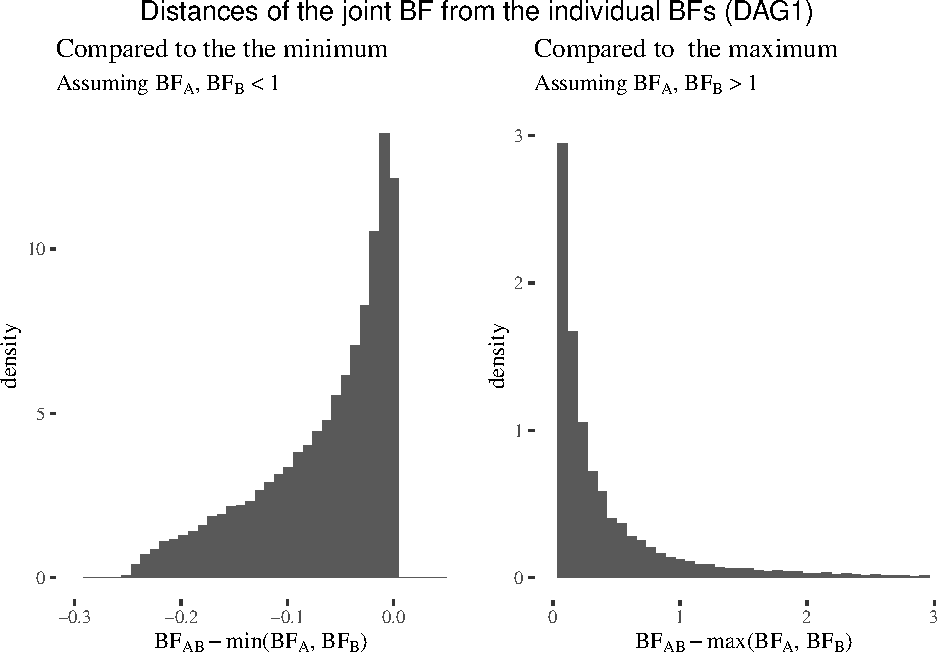
\includegraphics[width=1\linewidth]{conjunction-appendix7_files/figure-latex/BFind-1} \end{center}
\caption{Distances of the joint Bayes factor from maxima and minima of individual Bayes factors, depending on whether the individual support levels are both positive or both negative. Simulation based on 100k Bayesian networks build over the DAG of \textsf{DAG1}.}
\end{figure}

For the DAG corresponding to \textsf{DAG1}, the simulated frequency of
cases in which \(BF_{AB} < BF_{A}, BF_{B}\) is 25\% (which is twice
higher than for the likelihood ratio), and the structure of such cases
is visualized in Figure \ref{fig:BFfails}.

\begin{figure}

\begin{center}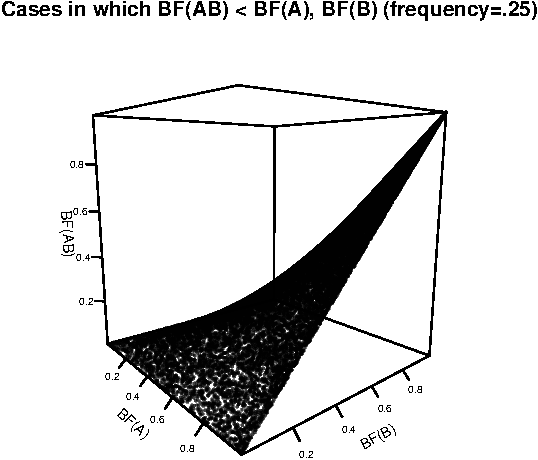
\includegraphics[width=1\linewidth]{conjunction-appendix7_files/figure-latex/unnamed-chunk-7-1} \end{center}
\caption{Ca. 25k cases (out of simulated 100k) in which the joint BF is below each of the individual BFs.}
\label{fig:BFfails}
\end{figure}

The picture doesn't change when we move to \textsf{DAG2} (Figure
\ref{fig:BFind2}). What does change, however, is that the joint BF is no
longer the result of multiplying the individual BFs. Nevertheless, the
values are fairly close (Figure \ref{fig:BFmulti}).

\vspace{1mm}
\footnotesize

\normalsize

\begin{figure}[ht]

\begin{center}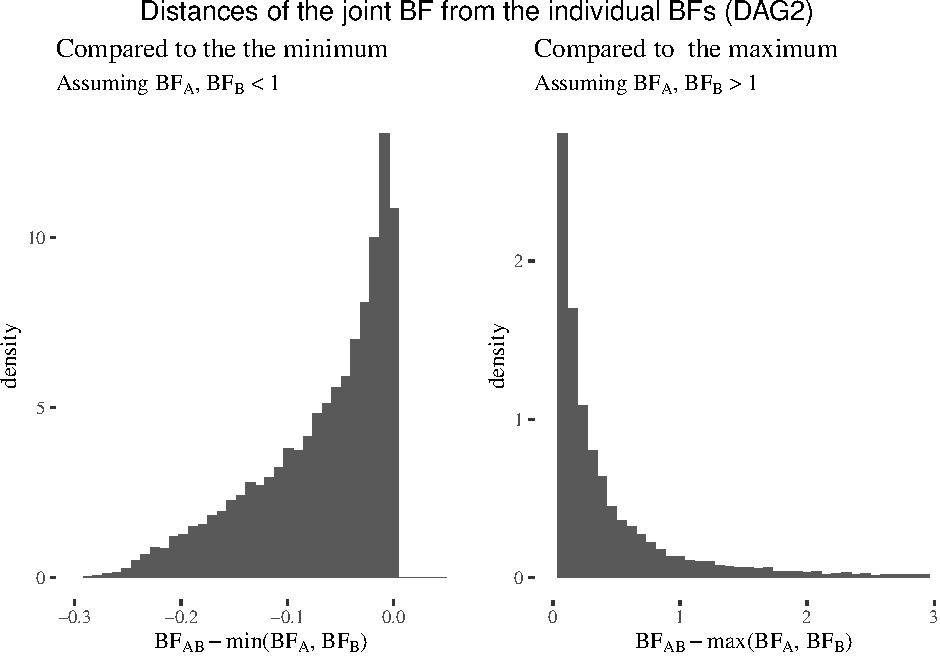
\includegraphics[width=1\linewidth]{conjunction-appendix7_files/figure-latex/BFind2-1} \end{center}

\caption{Distances of the joint Bayes factor from maxima and minima of individual Bayes factors, depending on whether the individual support levels are both positive or both negative. Simulation based on 100k Bayesian networks build over the DAG of \textsf{DAG2}.}
label{fig:BFind2}
\end{figure}

\begin{figure}[ht]

\begin{center}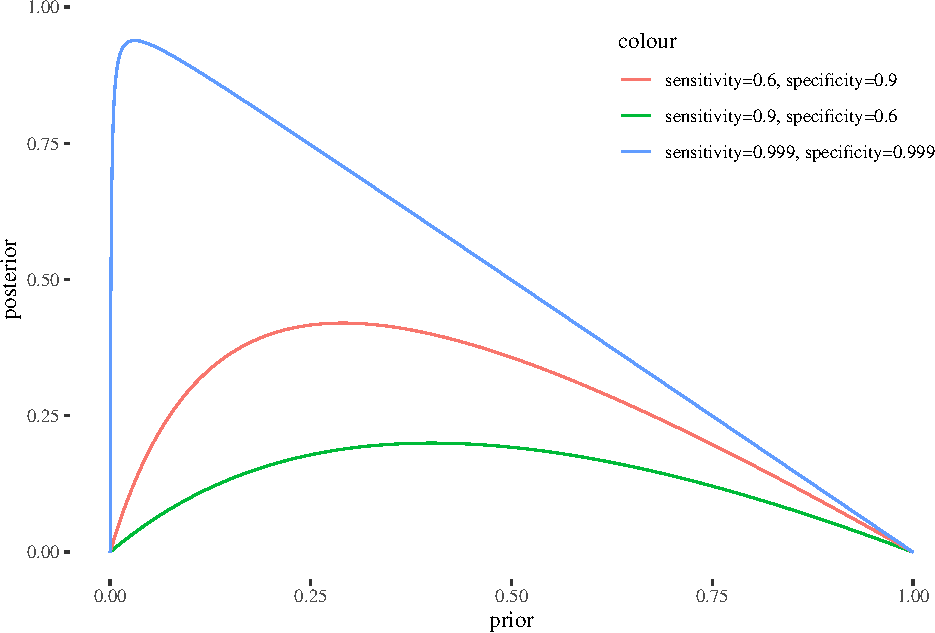
\includegraphics[width=1\linewidth]{conjunction-appendix7_files/figure-latex/unnamed-chunk-9-1} \end{center}
\caption{In DAG2, the result of multiplying individual BFs does not equal the joing BF, but often is a good approximation thereof.}
\label{fig:BFmulti}
\end{figure}

\hypertarget{likelihood-ratio-claims-and-proofs}{%
\subsection*{Likelihood ratio: claims and
proofs}\label{likelihood-ratio-claims-and-proofs}}
\addcontentsline{toc}{subsection}{Likelihood ratio: claims and proofs}

Now, let's turn to the likelihood understood as:

\begin{align*}
\frac{\pr{E \vert H}}{\pr{E \vert \neg H}} & =
\frac{\textit{sensitivity}}{\textit{1- specificity}}\end{align*}

\noindent Let's introduce the following abbreviations: \begin{align*}
LR_{AB} &= \frac{\pr{a\wedge b \vert a\wedge B}}{\pr{a \wedge b \vert \neg (A\wedge B)}}\\
LR_A & = \frac{\pr{a \vert A}}{\pr{a \vert \n A}} \\
LR_B & = \frac{\pr{b \vert B}}{\pr{b \vert \n B}}.
\end{align*}

\begin{fact} If independence conditions  \eqref{eq:I4}, \eqref{eq:I4a}, \eqref{eq:I4b},   \eqref{eq:I4c},  \eqref{eq:I5},   \eqref{eq:I5a},    \eqref{eq:I5b}, and   \eqref{eq:I5c}    hold, then:
\begin{align*}
LR_{AB} & =  \frac{\pr{a \vert A} \times \pr{b \vert B}}
 {\frac{\pr{\neg A}\pr{B \vert \neg A} \pr{a \vert \neg A}\pr{b \vert B} + \pr{A}\pr{\neg B \vert A} \pr{a \vert A }\pr{b \vert \neg B} + \pr{\neg A}\pr{\neg B \vert \neg A } \pr{a \vert \neg A}\pr{b \vert \neg B}}{\pr{\neg A}\pr{B \vert \neg A} + \pr{A}\pr{\neg B \vert A } + \pr{\neg A}\pr{\neg B \vert \neg A} }}
\end{align*}
\end{fact}

\noindent Note that these independence assumptions are entailed not only
in \textsf{DAG1}, but also in \textsf{DAG2}.

\begin{proof}
Let's first compute the numerator of $LR_{AB}$:

\begin{align*}
\pr{a \wedge b\vert A\wedge B} & =  \frac{\pr{A \et B \et a\et b}}{\pr{A \et B}}
&\mbox{(conditional probability)}
\\
&= \frac{   \pr{A} \times \pr{B\vert A} \times \pr{a \vert A \wedge B} \times \pr{b \vert A \wedge B \wedge a} }{\pr{A} \times \pr{B \vert A}}
&\mbox{(chain rule)}
\end{align*}

We deploy the relevant independencies as follows:
\begin{align*}
\mbox{      } &= \frac{   \pr{A} \times \pr{B\vert A} \times \overbrace{\pr{a \vert A \wedge B}}^{\pr{a \vert A} \mbox{ \footnotesize \, by \eqref{eq:I4} } } \times \overbrace{\pr{b \vert A \wedge B \wedge a}}^{\pr{b \vert B} \mbox{ \footnotesize \, by \eqref{eq:I5} }} }{\pr{A} \times \pr{B \vert A}}
&\mbox{}\\
 & = \pr{a \vert A} \times \pr{b \vert B} 
 &\mbox{(algebraic manipulation)} 
\end{align*}





\noindent The denominator of $LR_{AB}$ is more complicated, mostly because of the conditioning on  $\neg (A \wedge B)$.

\scalebox{.85}{\parbox{1\linewidth}{
\begin{align*}
\pr{a \et b\vert \neg (A\et B)} & = \frac{\pr{a \et b \et \neg (A\et B)}}{\pr{\neg (A \et B)}} 
&\mbox{ (conditional probability)}\\
& = \frac{\pr{a \et b \et \neg A\et B} +  \pr{a \et b \et A\et \neg B} + \pr{a \et b \et \neg A\et \neg B}  }{\pr{\neg A \et B} + \pr{A \et \neg B} + \pr{\neg A \et \neg B} } 
&\mbox{ (logic \& additivity)}
\end{align*}
}}



\noindent Now consider the first summand from the numerator:
\begin{align*}
\pr{a \et b \et \neg A\et B} & = \pr{\n A} \pr{B \vert \n A} \pr{a \vert \n A \et B} \pr{b\vert a \et \n A \et B} &\mbox{\,\,\,\,\,\,\,\,\,\,\,\,\, (chain rule)} \\ & = 
\pr{\neg A}\pr{B \vert \neg A} \pr{a \vert \neg A}\pr{b \vert B}
&\mbox{\,\,\,\,\,\,\,\,\,\,\,\,\, (independencies \eqref{eq:I4a} and \eqref{eq:I5a})} \\
\end{align*}

The simplification of the other two summanda is analogous (albeit with slightly different independence assumptions---\eqref{eq:I4b} and \eqref{eq:I5b} for the second one and \eqref{eq:I4c} and \eqref{eq:I5c} for the third. Once we plug these into the denominator formula we get:

\scalebox{.8}{\parbox{1\linewidth}{
\begin{align*}
\pr{a \et b\vert \neg (A\et B)} & = \frac{\pr{\neg A}\pr{B \vert \neg A} \pr{a \vert \neg A}\pr{b \vert B} + \pr{A}\pr{\neg B \vert A} \pr{a \vert A }\pr{b \vert \neg B} + \pr{\neg A}\pr{\neg B \vert \neg A } \pr{a \vert \neg A}\pr{b \vert \neg B}}{\pr{\neg A}\pr{B \vert \neg A} + \pr{A}\pr{\neg B \vert A } + \pr{\neg A}\pr{\neg B \vert \neg A} } \\
 & = \frac{\pr{\neg A}\pr{B \vert \neg A} \pr{a \vert \neg A}\pr{b \vert B} + \pr{A}\pr{\neg B \vert A} \pr{a \vert A }\pr{b \vert \neg B} + \pr{\neg A}\pr{\neg B \vert \neg A } \pr{a \vert \neg A}\pr{b \vert \neg B}}{\pr{\neg A}\pr{B \vert \neg A} + \pr{A}\pr{\neg B \vert A } + \pr{\neg A}\pr{\neg B \vert \neg A} }  
 \end{align*}}}

\end{proof}

\hypertarget{likelihod-ratio-simulations}{%
\subsection*{Likelihod ratio:
simulations}\label{likelihod-ratio-simulations}}
\addcontentsline{toc}{subsection}{Likelihod ratio: simulations}

While the analytic approach turns out to be cumbersome, let's inspect
the problem using simulations. First of all, there are cases in which
the joint likelihood ratio are lower than each of the individual
likelihood ratios. Their frequency is twice lower than the corresponding
frequency for the Bayes factor (recall Figure \ref{fig:BFfails}). For
the DAG corresponding to both \textsf{DAG}s, the simulated frequency of
cases in which \(LR_{AB} < LR_{A}, LR_{B}\) is 12-12.5\% and the
distribution of such cases, somewhat of a different shape, is visualized
in Figure \ref{fig:LRfails} (the picture for \textsf{DAG2} is very
similar).

\begin{figure}

\begin{center}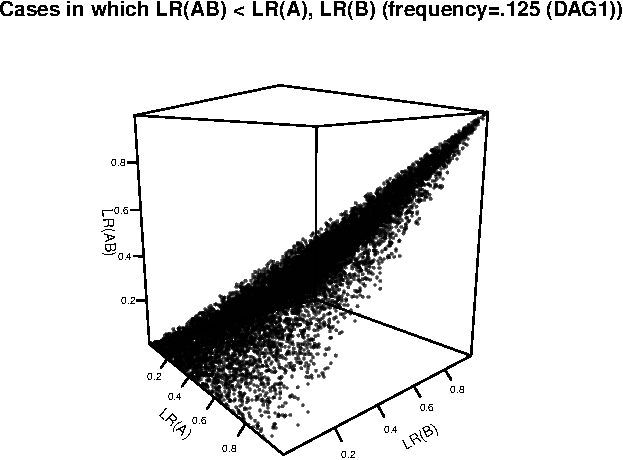
\includegraphics[width=1\linewidth]{conjunction-appendix7_files/figure-latex/unnamed-chunk-10-1} \end{center}
\caption{Ca. 25k cases (out of simulated 100k) in which the joint BF is below each of the individual BFs.}
\label{fig:LRfails}
\end{figure}

Interestingly, even if the individual likelihood ratios are \(<1\), the
joint likelihood ratio can be higher than their minimum, but is never
higher than their maximum (Figure \ref{fig:LRlowerPlot}).

\vspace{1mm}
\footnotesize

\begin{center}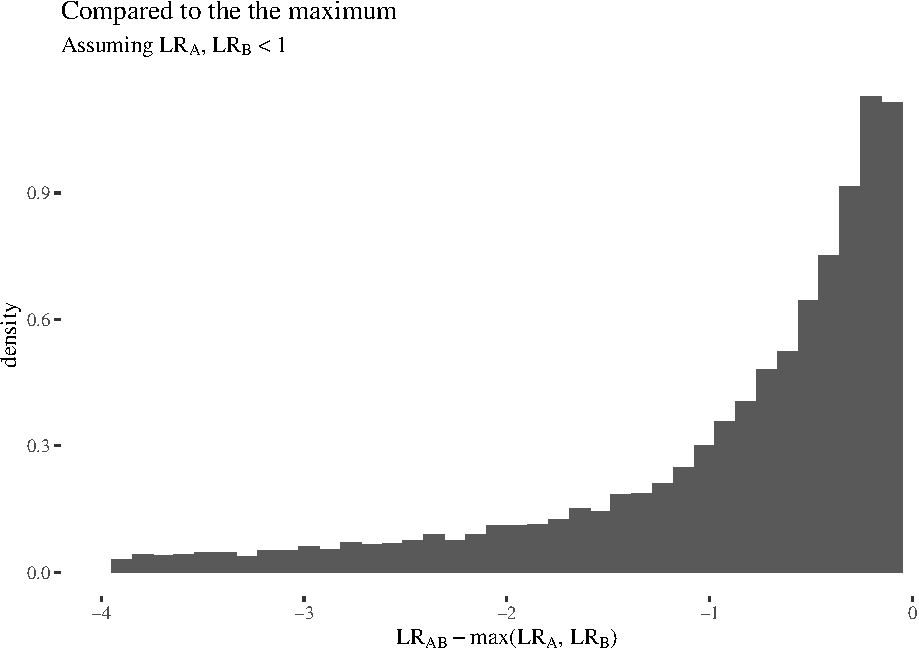
\includegraphics[width=1\linewidth]{conjunction-appendix7_files/figure-latex/unnamed-chunk-11-1} \end{center}
\normalsize

\begin{figure}


\begin{center}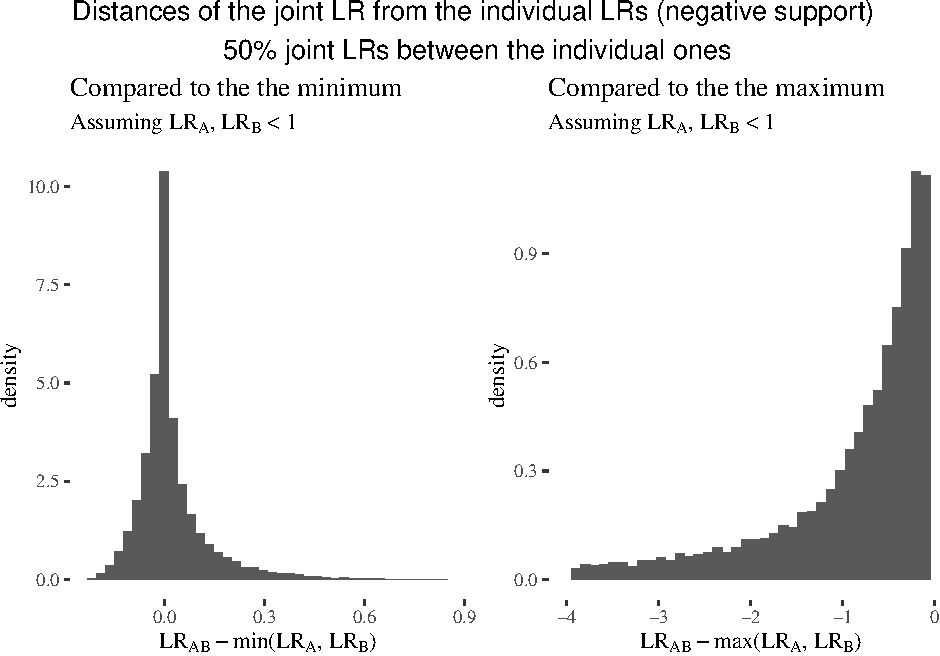
\includegraphics[width=1\linewidth]{conjunction-appendix7_files/figure-latex/unnamed-chunk-12-1} \end{center}

\caption{Distances of joint likelihood ratios for the minima and the maxima of the individual likelihood ratios if the individual likelihood ratios are below 1, DAG used in \textsf{DAG1}.} 
\label{fig:LRlowerPlot}
\end{figure}

Once the individual likelihood ratios are above 1, the joint likelihood
ratio can be lower than the maximum, but is not lower than the minimum
of the individual likelihood ratios (Figure \ref{fig:LRabovePlot}).

\begin{figure}


\begin{center}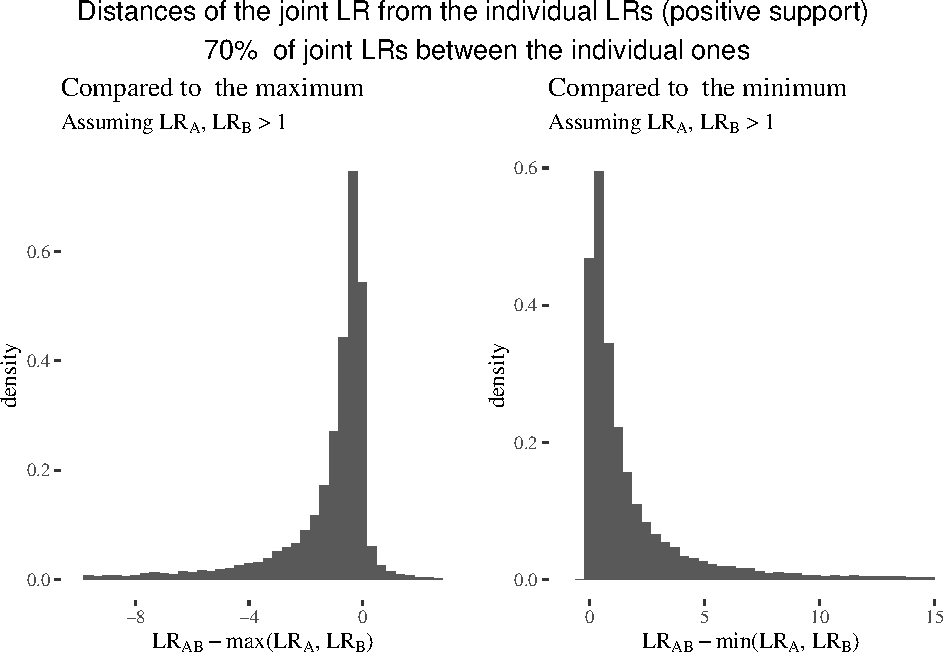
\includegraphics[width=1\linewidth]{conjunction-appendix7_files/figure-latex/unnamed-chunk-13-1} \end{center}

\caption{Distances of joint likelihood ratios for the minima and the maxima of the individual likelihood ratios if the individual likelihood ratios are above 1, DAG used in \textsf{DAG1}.}
\label{fig:LRabovePlot}
\end{figure}

\end{document}
